\chapter{Experimental Results and Performance Evaluation}\label{ch:results}

\section{Introduction}\label{sec:res-intro}
This chapter evaluates the two controllers of Chapter~\ref{ch:proposed}. The experiments ask, for each controller, whether replacing fixed settings by the frozen controller improves tracking with the same detector and tracker, and whether it keeps this effect on data that were not used to build it. Section~\ref{sec:res-setup} describes the datasets, the evaluation metrics, the statistical comparison, and the implementation environment. Section~\ref{sec:res-acmot} gives the results of AC-MOT on VisDrone2019-MOT and, without retuning, on UAVDT. Section~\ref{sec:res-scl} gives the results of SCL on seven published trackers under detector and score changes, on predeclared external trackers, and on a held-out aerial test split. Section~\ref{sec:res-compare} compares the proposed controllers with existing approaches, and Section~\ref{sec:res-discussion} discusses the results.

\section{Setup Discussion}\label{sec:res-setup}

\subsection{Datasets}\label{sec:res-datasets}
Four public datasets are used. Table~\ref{tab:res-data} lists the splits and the role of each one.

\emph{VisDrone2019-MOT.} VisDrone2019-MOT is a widely used benchmark for MOT in UAV videos \cite{zhu2022visdrone}. It contains video sequences recorded by various drone-mounted cameras in 14 cities in China, in urban and rural regions and in both sparse and crowded scenes. The VisDrone benchmark annotates ten object categories, such as pedestrians, cars, buses, and bicycles, with boxes that give the location and identity of each tracked object. Its MOT track uses 96 video clips: 56 for training (24,198 frames), 7 for validation (2,846 frames), 16 for challenge testing (6,322 frames), and 17 for development testing (6,635 frames). Although ten categories are annotated, the official MOT evaluation scores only five of them: pedestrian, car, van, bus, and truck \cite{zhu2022visdrone}. Many objects are small, their number changes quickly in crowded traffic, the moving camera changes position and viewing angle, and lighting, background, and occlusion vary. These properties make the dataset suitable for studying detector settings. Eight training clips serve as calibration data for AC-MOT (Section~\ref{sec:ac-modern}), and the seven validation clips serve as its evaluation data.

\emph{UAVDT.} UAVDT is a benchmark designed for object detection and MOT in UAV videos, with a particular focus on vehicles \cite{du2018uavdt}. It consists of 100 video sequences selected from more than 10 hours of video recorded at urban locations such as squares, arterial streets, toll stations, highways, crossings, and T-junctions, at 30 frames per second and a resolution of $1080\times540$ pixels. About 80,000 frames are annotated with 0.84 million boxes of vehicles in three categories: car, truck, and bus. The sequences are recorded under different weather conditions, flying altitudes, and camera viewing angles, which change object size, visibility, and the number of vehicles per frame. The test set contains 20 sequences for the MOT task (16,592 frames) \cite{du2018uavdt}. These 20 sequences are used by both controllers, with all vehicles in one class.

\emph{MOT17.} MOT17 \cite{milan2016mot16} contains 14 sequences of people filmed with static and moving cameras. As is common, the second half of each of the seven training sequences, called val-half (2,652 frames), is used for evaluation \cite{zhang2022bytetrack}, with the published YOLOX-X detections \cite{ge2021yolox} at the two published emission floors, the lowest scores emitted, of 0.01 and 0.1. To study score changes directly, these scores were also changed before the tracker by four transforms that keep their order: cubing ($s^3$), halving ($0.5\,s$), and logit temperatures $T=2$ and $T=0.5$, which divide the logit of each score by $T$.

\emph{KITTI tracking.} KITTI tracking \cite{geiger2012kitti} has 21 training sequences (8,008 frames) recorded from a car and is scored on cars and pedestrians. Here the trackers run with two other detectors, YOLOv8n \cite{jocher2023yolov8} and RT-DETR-L \cite{zhao2024rtdetr}, and keep thresholds that were set for other detectors.

For SCL, MOT17 with four trackers, KITTI, and the score transforms were development data, looked at while the layer was designed. Two predeclared external trackers, PD-SORT and Hybrid-SORT, were chosen in advance and run once with the frozen configuration on the detections released by their authors on MOT17 val-half. The held-out UAVDT test split was also run once, after a written plan. Each external host was checked against its authors' number: EXACT within 0.2 HOTA points, CLOSE within 1.0.

\begin{table}[tbp]
\centering
\caption{Datasets and splits used in the experiments and the role of each one.}
\label{tab:res-data}
\begin{tabular}{>{\raggedright\arraybackslash}p{3.0cm}>{\raggedright\arraybackslash}p{4.8cm}>{\raggedright\arraybackslash}p{1.7cm}>{\raggedright\arraybackslash}p{4.8cm}}
\toprule
Dataset & Split & Controller & Role\\
\midrule
VisDrone2019-MOT & training, 8 sequences (3,282 frames) & AC-MOT & calibration (tuning) data\\
VisDrone2019-MOT & validation, 7 sequences (2,846 frames) & AC-MOT & frozen evaluation\\
UAVDT & test, 20 sequences (16,592 frames) & AC-MOT & transfer without retuning\\
MOT17 & val-half, 7 sequences (2,652 frames) & SCL & development; predeclared external trackers\\
KITTI tracking & training, 21 sequences (8,008 frames) & SCL & development under a detector change\\
UAVDT & test, 20 sequences (16,592 frames) & SCL & held-out evaluation, run once\\
\bottomrule
\end{tabular}
\end{table}

\subsection{Evaluation Metrics}\label{sec:res-metrics}
Eight commonly used MOT metrics are considered: HOTA, MOTA, IDF1, identity switches (IDS), false positives (FP), false negatives (FN), precision, and recall. These metrics measure different aspects of tracking performance, including detection accuracy, object identity consistency, and the ability to track objects across consecutive frames \cite{dendorfer2021motchallenge,luiten2021hota}. They are defined below, starting from the errors counted in each frame and ending with the scores that combine them.

\emph{Detection errors.} The first metrics count the errors made frame by frame. In each frame $t$, output boxes are matched one to one to ground-truth boxes with an IoU of at least 0.5. Let $\mathrm{GT}_t$ be the number of ground-truth boxes, $\mathrm{TP}_t$ the number of matched pairs, $\mathrm{FP}_t$ the number of output boxes without a match (false positives), and $\mathrm{FN}_t$ the number of ground-truth boxes without a match (false negatives, or missed objects). Over all frames,
\begin{align}
\mathrm{GT}&=\sum_t \mathrm{GT}_t,\qquad \mathrm{TP}=\sum_t \mathrm{TP}_t,\label{eq:res-gt}\\
\mathrm{FP}&=\sum_t \mathrm{FP}_t,\qquad \mathrm{FN}=\sum_t \mathrm{FN}_t,\label{eq:res-fpfn}
\end{align}
so that $\mathrm{TP}=\mathrm{GT}-\mathrm{FN}$. From these counts, precision is the fraction of output boxes that are correct, and recall is the fraction of ground-truth boxes that are found:
\begin{equation}
\mathrm{Precision}=\frac{\mathrm{TP}}{\mathrm{TP}+\mathrm{FP}},\qquad
\mathrm{Recall}=\frac{\mathrm{TP}}{\mathrm{GT}}.
\label{eq:res-prrc}
\end{equation}

\emph{Identity switches.} The counts above treat each frame separately, so they do not show whether an object keeps the same track over time. Identity switches measure this. Let $\phi_t(i)$ be the output track matched to ground-truth object $i$ in frame $t$, and $\phi_{\mathrm{prev}}(i)$ the output track to which object $i$ was last matched before $t$. An identity switch is counted whenever these two tracks differ:
\begin{equation}
\mathrm{IDS}=\sum_t\sum_{i}\mathbf{1}\!\left[\phi_t(i)\neq\phi_{\mathrm{prev}}(i)\right],
\label{eq:res-ids}
\end{equation}
where the inner sum runs over the objects that are matched in frame $t$ and were matched before.

\emph{MOTA and IDF1.} These two scores summarize the errors above in a single number each \cite{bernardin2008clear,ristani2016idf1}. MOTA combines the three error types, and IDF1 measures how long each object keeps the correct identity:
\begin{align}
\mathrm{MOTA}&=1-\frac{\mathrm{FN}+\mathrm{FP}+\mathrm{IDS}}{\mathrm{GT}},\label{eq:res-mota}\\
\mathrm{IDF1}&=\frac{2\,\mathrm{IDTP}}{2\,\mathrm{IDTP}+\mathrm{IDFP}+\mathrm{IDFN}}.\label{eq:res-idf1}
\end{align}
For IDF1, each ground-truth track is first matched to at most one output track over the whole video. IDTP, IDFP, and IDFN are then the true-positive, false-positive, and false-negative boxes under this track-level matching. Because MOTA counts every false positive and every missed object, it reacts strongly to how many boxes the detector passes on. IDF1 depends more on whether each object keeps one identity.

\emph{HOTA.} MOTA depends mostly on detection errors, and IDF1 mostly on identity errors. HOTA balances detection and association in one score \cite{luiten2021hota}. At a localization threshold $\alpha$, let $\mathrm{TP}_\alpha$, $\mathrm{FN}_\alpha$, and $\mathrm{FP}_\alpha$ be the matched pairs, missed ground-truth boxes, and unmatched output boxes. For a matched pair $c$, $\mathrm{TPA}(c)$ is the set of matched pairs with the same ground-truth identity and the same output identity as $c$; $\mathrm{FNA}(c)$ is the set of boxes of the same ground-truth object that are matched to another output identity or not matched; and $\mathrm{FPA}(c)$ is the set of boxes of the same output track that are matched to another object or not matched. Then
\begin{align}
\mathrm{DetA}_\alpha&=\frac{|\mathrm{TP}_\alpha|}{|\mathrm{TP}_\alpha|+|\mathrm{FN}_\alpha|+|\mathrm{FP}_\alpha|},\label{eq:res-deta}\\
\mathcal{A}(c)&=\frac{|\mathrm{TPA}(c)|}{|\mathrm{TPA}(c)|+|\mathrm{FNA}(c)|+|\mathrm{FPA}(c)|},\label{eq:res-ac}\\
\mathrm{AssA}_\alpha&=\frac{1}{|\mathrm{TP}_\alpha|}\sum_{c\in\mathrm{TP}_\alpha}\mathcal{A}(c),\label{eq:res-assa}\\
\mathrm{HOTA}&=\frac{1}{19}\sum_{\alpha}\sqrt{\mathrm{DetA}_\alpha\,\mathrm{AssA}_\alpha},\label{eq:res-hota}
\end{align}
where $\alpha$ runs over $0.05, 0.10, \dots, 0.95$; $\mathrm{DetA}$ is the detection accuracy and $\mathrm{AssA}$ the association accuracy.

\emph{Evaluation tools.} For AC-MOT on VisDrone, results are scored with a Python port of the VisDrone2019-MOT Task~4b evaluation: ignored regions are removed, the five classes are evaluated separately, CLEAR-MOT and identity measures use IoU 0.5, and counts are summed over classes and sequences; HOTA is added with the same class-aware scheme using TrackEval. For SCL, all metrics are computed with TrackEval (commit 12c8791) and the official ground truth \cite{dendorfer2021motchallenge}; KITTI HOTA is averaged over cars and pedestrians. On UAVDT all vehicles form one class and predictions in ignored regions are removed.

\emph{Units and direction.} HOTA, MOTA, IDF1, precision, and recall are given in percent, and differences in points; IDS, FP, and FN are counts; speed is given in FPS, and runtime in milliseconds (ms) per frame. Higher values are better for HOTA, MOTA, IDF1, precision, recall, and FPS, and lower values are better for IDS, FP, FN, and runtime.

\subsection{Statistical Comparison}\label{sec:res-bootstrap}
All comparisons are paired: each tracker runs with fixed settings and with the controller on the same sequences and detections, and nothing else changes. To judge whether the difference between two systems is reliable, paired bootstrap resampling is applied at the sequence level \cite{efron1993bootstrap}, which keeps the dependence within each sequence. Each resample draws the evaluation sequences with replacement; the same draw is used for both systems, the pooled metrics are recomputed, and their difference is recorded. The 95\% interval is the 2.5--97.5 percentile range, and a difference is called significant when its interval does not include zero. The AC-MOT comparisons use 5000 resamples and the SCL comparisons 10,000 resamples, both with seed 42. Because whole sequences are resampled, the intervals reflect the variation between videos, not only between frames.

\subsection{Implementation Environment and Toolkit}\label{sec:res-env}
The controllers and the evaluation are implemented in Python. The image cues use OpenCV (the Canny edge detector, the Laplacian, and phase correlation) and NumPy; the detectors run with PyTorch and the Ultralytics library; the tracking metrics are computed with TrackEval; and the development searches of AC-MOT use Optuna \cite{akiba2019optuna}. Table~\ref{tab:res-env} summarizes the detectors, trackers, and hardware of each controller.

\emph{AC-MOT.} All experiments use the YOLO11m detector \cite{jocher2024yolo11} in a public version trained on VisDrone2019-DET. It runs in half precision, and detections of the classes pedestrian, car, van, truck, and bus are passed on. ByteTrack uses the Ultralytics implementation with its default parameters: high threshold 0.25, low threshold 0.10, new-track threshold 0.25, buffer 30 frames, and match threshold 0.80. OATrack is a re-implementation of the published method \cite{qi2026oatrack} in its main configuration, with its published tracker-side confidence gate of 0.40. This gate belongs to the tracker and is never changed by AC-MOT. For each host, two systems are compared. The baseline runs the detector at the fixed operating point of 1536 pixels and NMS IoU 0.70, with a minimal score threshold of 0.01 (Section~\ref{sec:ac-constants}). AC-MOT runs the frozen controller of Section~\ref{sec:acmot} on the same detector, so the two systems differ only in the detector operating point. Latency is measured on one Tesla T4 GPU over the first 200 frames of sequence uav0000086\_00000\_v, excluding five warm-up frames. For every frame, the time spent in the controller (image statistics, scene analysis, and state update) is recorded separately from the detector and tracker time.

\emph{SCL.} Seven published trackers serve as hosts, each with the authors' code and published configuration: ByteTrack \cite{zhang2022bytetrack}, BoT-SORT \cite{aharon2022botsort}, OC-SORT \cite{cao2023ocsort}, SparseTrack \cite{liu2025sparsetrack}, BoostTrack \cite{stanojevic2024boosttrack}, PD-SORT \cite{wang2025pdsort}, and Hybrid-SORT \cite{yang2024hybridsort}. ByteTrack is used with the thresholds that its authors used on MOT17 (official setting) and with the defaults of the Ultralytics library, which also provides BoT-SORT (library setting). For each host, the baseline is the host alone (Host in the tables), run with its published configuration and the same detections; the second run adds the frozen SCL and changes nothing else. The runtime of SCL is measured on a 4-vCPU Intel Xeon processor at 2.10 GHz without a GPU, with YOLOv8n and ByteTrack on three KITTI sequences (2,279 timed frames).

\begin{table}[tbp]
\centering
\caption{Detectors, trackers, data, and hardware used to evaluate the two controllers.}
\label{tab:res-env}
\begin{tabular}{>{\raggedright\arraybackslash}p{2.8cm}>{\raggedright\arraybackslash}p{5.6cm}>{\raggedright\arraybackslash}p{5.9cm}}
\toprule
Item & AC-MOT & SCL\\
\midrule
Detectors & YOLO11m (VisDrone2019-DET weights), half precision & YOLOX-X (published MOT17 detections), YOLOv8n, RT-DETR-L\\
Trackers & ByteTrack (Ultralytics), OATrack & ByteTrack, BoT-SORT, OC-SORT, SparseTrack, BoostTrack, PD-SORT, Hybrid-SORT\\
Data & VisDrone2019-MOT, UAVDT & MOT17, KITTI tracking, UAVDT\\
Baseline & fixed operating point (1536, 0.70) & host alone with its published configuration\\
Bootstrap & 5000 resamples, seed 42 & 10,000 resamples, seed 42\\
Runtime hardware & Tesla T4 GPU & 4-vCPU Intel Xeon at 2.10 GHz, no GPU\\
\bottomrule
\end{tabular}
\end{table}

\section{Results of the Scene-Adaptive Controller (AC-MOT)}\label{sec:res-acmot}

\subsection{Frozen VisDrone Evaluation}\label{sec:res-ac-visdrone}
The VisDrone evaluation uses seven sequences of the VisDrone2019-MOT validation split. They contain 71,830 ground-truth boxes. The cue subset, thresholds, and action map of the frozen controller were selected on the separate calibration sequences only (Section~\ref{sec:ac-modern}). The bootstrap draws seven sequences with replacement. Table~\ref{tab:res-ac-visdrone} lists the aggregate results on the seven VisDrone sequences, and Fig.~\ref{fig:res-ac-visdrone} shows HOTA, MOTA, and IDF1.

\begin{table}[tbp]
\centering
\caption{Frozen VisDrone evaluation on seven VisDrone2019-MOT sequences (71,830 ground-truth boxes). Baseline: fixed operating point (1536, 0.70).}
\label{tab:res-ac-visdrone}
\begin{tabular}{lrrrr}
\toprule
 & \multicolumn{2}{c}{ByteTrack} & \multicolumn{2}{c}{OATrack}\\
Metric & Baseline & AC-MOT & Baseline & AC-MOT\\
\midrule
HOTA & 41.586 & 44.523 & 46.770 & 48.095\\
MOTA & 9.876 & 27.871 & 28.165 & 34.483\\
IDF1 & 48.569 & 53.929 & 57.107 & 59.364\\
IDS & 1341 & 1016 & 773 & 604\\
FP & 39274 & 24892 & 25394 & 21400\\
FN & 24121 & 25902 & 25432 & 25057\\
Precision & 54.849 & 64.852 & 64.628 & 68.609\\
Recall & 66.419 & 63.940 & 64.594 & 65.116\\
\bottomrule
\end{tabular}
\end{table}

\emph{ByteTrack host.} AC-MOT raises HOTA, MOTA, and IDF1 and lowers IDS and FP, while FN rise from 24121 to 25902 and recall falls from 66.419 to 63.940. The detector output becomes more selective: clutter and identity-confusing boxes are removed at a small cost in recall. The very low baseline MOTA shows how many FP the fixed operating point passes to this tracker; because MOTA counts every FP, the removal of more than a third of them is the main source of the MOTA gain.

\emph{OATrack host.} OATrack starts from a stronger baseline, and its gains are smaller, but every metric of Table~\ref{tab:res-ac-visdrone} moves in the direction of improvement, including FN (25432 to 25057) and recall (64.594 to 65.116).

\begin{figure}[tbp]
\centering
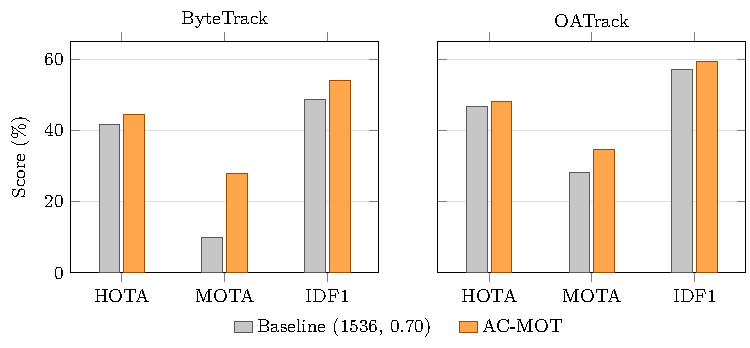
\includegraphics[width=0.85\textwidth]{figures/acmot_visdrone_bars.pdf}
\caption{HOTA, MOTA, and IDF1 on the seven VisDrone sequences for both tracker hosts (values in Table~\ref{tab:res-ac-visdrone}).}
\label{fig:res-ac-visdrone}
\end{figure}

\emph{Paired bootstrap.} In the VisDrone columns of Table~\ref{tab:res-ac-bootstrap}, the ByteTrack intervals of HOTA, MOTA, IDF1, precision, IDS, and FP lie entirely on the side of improvement, while FN and recall move in the opposite direction. With OATrack, HOTA, MOTA, IDF1, and precision rise and IDS and FP fall, all with intervals on one side of zero.

\begin{table}[tbp]
\centering
\caption{Paired sequence-level bootstrap of AC-MOT: AC-MOT minus baseline, 5000 resamples, seed 42, on VisDrone (7 sequences) and UAVDT (20 sequences). HOTA, MOTA, IDF1, precision, and recall in points; IDS, FP, and FN in counts. On UAVDT the bootstrap covers the count-based metrics only.}
\label{tab:res-ac-bootstrap}
\begin{tabular}{llrlrl}
\toprule
 & & \multicolumn{2}{c}{VisDrone} & \multicolumn{2}{c}{UAVDT}\\
Host & Metric & Difference & 95\% interval & Difference & 95\% interval\\
\midrule
ByteTrack & HOTA & $+2.937$ & [$+2.356$, $+3.375$] & -- & \\
 & MOTA & $+17.995$ & [$+13.541$, $+23.282$] & $+17.601$ & [$+11.134$, $+26.767$]\\
 & IDF1 & $+5.360$ & [$+4.490$, $+6.178$] & $+3.367$ & [$+1.676$, $+5.013$]\\
 & IDS & $-325$ & [$-498$, $-164$] & $-115$ & [$-211.025$, $-26.975$]\\
 & FP & $-14382$ & [$-19176$, $-9620$] & $-67539$ & [$-104215.350$, $-37352.950$]\\
 & FN & $+1781$ & [$+288$, $+3594.075$] & $+7652$ & [$+1542.925$, $+18359.400$]\\
 & Precision & $+10.003$ & [$+8.712$, $+11.895$] & -- & \\
 & Recall & $-2.479$ & [$-4.507$, $-0.469$] & -- & \\
\midrule
OATrack & HOTA & $+1.325$ & [$+0.200$, $+2.264$] & -- & \\
 & MOTA & $+6.318$ & [$+4.741$, $+7.879$] & $+3.267$ & [$+0.607$, $+5.881$]\\
 & IDF1 & $+2.258$ & [$+0.548$, $+3.474$] & $+0.831$ & [$+0.125$, $+1.271$]\\
 & IDS & $-169$ & [$-292$, $-42$] & $-31$ & [$-101$, $+39$]\\
 & FP & $-3994$ & [$-6190$, $-2494.900$] & $-14268$ & [$-33958.075$, $-2188.950$]\\
 & FN & $-375$ & [$-1462.575$, $+670$] & $+3162$ & [$-211.100$, $+8959.050$]\\
 & Precision & $+3.981$ & [$+2.957$, $+5.511$] & -- & \\
 & Recall & $+0.522$ & [$-0.869$, $+2.111$] & -- & \\
\bottomrule
\end{tabular}
\end{table}

\subsection{Controller Behavior}\label{sec:res-ac-behavior}
The controller uses all three states with both hosts. With ByteTrack, LOW, MEDIUM, and HIGH cover 7.4\%, 30.1\%, and 62.5\% of the frames; with OATrack they cover 7.4\%, 33.3\%, and 59.3\%. For most of the video, the detector therefore runs with the HIGH action, the smallest input and a score threshold of 0.40. The two hosts diverge through their different tracked boxes. State changes are rare, between 0.10 and 0.54 per 100 frames depending on the sequence, so the detector input stays stable over long stretches of video.

\subsection{Frozen UAVDT Transfer}\label{sec:res-ac-uavdt}
The UAVDT transfer tests whether the frozen controller still helps on a different dataset with none of its values changed. It uses 20 test sequences with 16,592 frames, scored with one vehicle class. Detector outputs were produced at the three frozen operating points (49,776 detector forward passes), with a single frozen run per host. The paired bootstrap draws 20 sequences with replacement from the stored per-sequence counts and therefore covers the count-based metrics MOTA, IDF1, IDS, FP, and FN.

\begin{table}[tbp]
\centering
\caption{Frozen UAVDT transfer of AC-MOT without retuning (20 sequences, 16,592 frames, one vehicle class). Baseline: fixed operating point (1536, 0.70).}
\label{tab:res-ac-uavdt}
\begin{tabular}{lrrrr}
\toprule
 & \multicolumn{2}{c}{ByteTrack} & \multicolumn{2}{c}{OATrack}\\
Metric & Baseline & AC-MOT & Baseline & AC-MOT\\
\midrule
HOTA & 45.923 & 47.004 & 47.728 & 47.640\\
MOTA & $-1.573$ & 16.028 & 19.607 & 22.873\\
IDF1 & 58.400 & 61.767 & 62.101 & 62.931\\
IDS & 601 & 486 & 517 & 486\\
FP & 279616 & 212077 & 197937 & 183669\\
FN & 66050 & 73702 & 75612 & 78774\\
Precision & 49.571 & 55.751 & 57.270 & 58.800\\
Recall & 80.625 & 78.381 & 77.820 & 76.893\\
\bottomrule
\end{tabular}
\end{table}

Table~\ref{tab:res-ac-uavdt} and Fig.~\ref{fig:res-ac-uavdt} report the transfer to UAVDT without retuning. With ByteTrack, HOTA rises by 1.081 points, MOTA by 17.601, and IDF1 by 3.367; with OATrack, MOTA rises by 3.267 and IDF1 by 0.831, while HOTA is almost unchanged (47.728 and 47.640). With both hosts FP and IDS fall and precision rises, with slightly lower recall, the same pattern as with ByteTrack on VisDrone: the controller changes the detector output in the same way on a dataset that was not used to build it.

In the UAVDT columns of Table~\ref{tab:res-ac-bootstrap}, the ByteTrack intervals of MOTA, IDF1, IDS, and FP lie on the side of improvement and FN moves the other way; with OATrack, MOTA and IDF1 rise and FP fall with intervals on one side of zero, while the IDS and FN intervals include zero.

\begin{figure}[tbp]
\centering
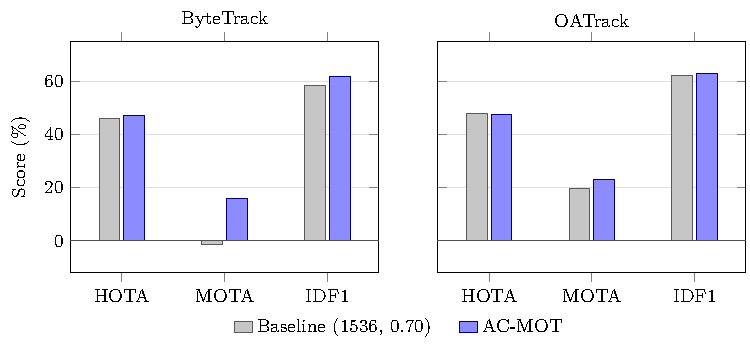
\includegraphics[width=0.85\textwidth]{figures/acmot_uavdt_bars.pdf}
\caption{HOTA, MOTA, and IDF1 of the frozen UAVDT transfer of AC-MOT for both tracker hosts (values in Table~\ref{tab:res-ac-uavdt}). The ByteTrack baseline MOTA is negative ($-1.573$); the solid line marks zero.}
\label{fig:res-ac-uavdt}
\end{figure}

\subsection{Runtime of AC-MOT}\label{sec:res-ac-runtime}
AC-MOT needs no training and no access to detector or tracker internals; it changes three arguments of the detector call and analyzes a quarter-scale image every ten frames. On a Tesla T4 the controller takes 4.26 ms per frame with ByteTrack and 4.20 ms with OATrack, which is small next to detector inference and suitable for real-time use.

\section{Results of the Self-Calibrating Control Layer (SCL)}\label{sec:res-scl}
A tracker that fits its detector should keep its accuracy, and one that does not, because it lacks a continuation step or because the detector or its scores changed, should gain. Figure~\ref{fig:res-scl-forest} summarizes the HOTA difference for every tested cell.

\begin{figure}[tbp]
\centering
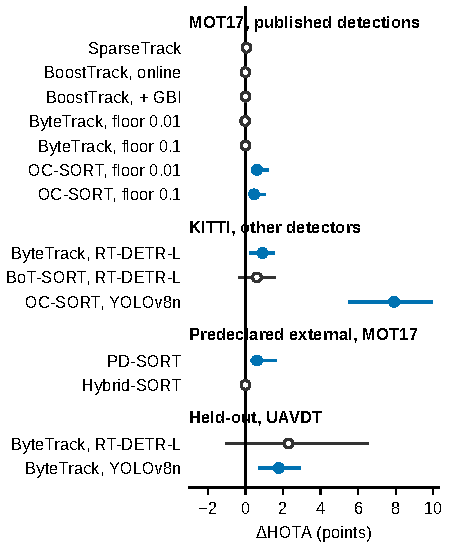
\includegraphics[width=0.62\textwidth]{figures/scl_forest.pdf}
\caption{Difference in HOTA, host with SCL minus host alone, in points, for every tested cell, with its 95\% paired-bootstrap interval. Filled circles: interval above zero; open circles: interval contains zero, or identical output.}
\label{fig:res-scl-forest}
\end{figure}

\subsection{MOT17 Evaluation Across Trackers}\label{sec:res-scl-mot17}
Table~\ref{tab:res-scl-mot17} shows the development trackers on MOT17 val-half. The two-stage trackers with well-matched detections stayed at the accuracy of their hosts: BoostTrack, online and with GBI, and ByteTrack at floor 0.1 gave exactly the same output, and ByteTrack at floor 0.01 and SparseTrack stayed within 0.06 HOTA points, the self-limiting clean mode. The single-stage OC-SORT improved at both floors (HOTA $+0.61$ and $+0.46$, MOTA $+1.27$ and $+1.26$), with fewer identity switches and higher HOTA on 7 of 7 sequences, through the continuation rescue.

\begin{table}[tbp]
\centering
\caption{Baseline comparison of the development trackers on MOT17 val-half (published YOLOX-X detections). Paper: number reported by the tracker's authors. Host: the tracker alone, without SCL (our run of the published tracker). $\Delta$: host with SCL minus host, with 95\% paired-bootstrap interval (10,000 resamples, seed 42); bold intervals exclude zero. The floor is the lowest detector score emitted. IDS: identity switches, a count (lower is better); --: not reported by the authors.}
\label{tab:res-scl-mot17}
\begin{tabular}{lrrl}
\toprule
Metric & Paper & Host & $\Delta$ [95\% CI]\\
\midrule
\multicolumn{4}{l}{\textit{SparseTrack} \cite{liu2025sparsetrack}}\\
\quad HOTA & 69.2 & 68.88 & $+0.06$ [$-0.01$, $+0.25$]\\
\quad MOTA & 76.8 & 77.85 & $+0.08$ [$-0.03$, $+0.30$]\\
\quad IDF1 & 81.4 & 81.97 & $+0.16$ [$-0.02$, $+0.70$]\\
\quad IDS & -- & 124 & $+7$ [$0$, $+19$]\\
\multicolumn{4}{l}{\textit{BoostTrack, online} \cite{stanojevic2024boosttrack}}\\
\quad HOTA & 68.37 & 68.49 & 0 (identical)\\
\quad MOTA & 75.56 & 75.50 & 0 (identical)\\
\quad IDF1 & 81.35 & 81.41 & 0 (identical)\\
\quad IDS & 118 & 113 & 0 (identical)\\
\multicolumn{4}{l}{\textit{BoostTrack, + GBI} \cite{stanojevic2024boosttrack}}\\
\quad HOTA & 71.33 & 71.72 & 0 (identical)\\
\quad MOTA & 80.55 & 81.03 & 0 (identical)\\
\quad IDF1 & 83.84 & 84.16 & 0 (identical)\\
\quad IDS & 106 & 97 & 0 (identical)\\
\multicolumn{4}{l}{\textit{ByteTrack, floor 0.01} \cite{zhang2022bytetrack}}\\
\quad HOTA & -- & 67.70 & $-0.014$ [$-0.058$, $+0.009$]\\
\quad MOTA & 76.6 & 77.60 & $+0.06$ [$-0.15$, $+0.34$]\\
\quad IDF1 & 79.3 & 79.47 & $-0.031$ [$-0.135$, $+0.035$]\\
\quad IDS & -- & 214 & $+4$ [$-2$, $+13$]\\
\multicolumn{4}{l}{\textit{ByteTrack, floor 0.1} \cite{zhang2022bytetrack}}\\
\quad HOTA & -- & 67.70 & 0 (identical)\\
\quad MOTA & 76.6 & 77.60 & 0 (identical)\\
\quad IDF1 & 79.3 & 79.47 & 0 (identical)\\
\quad IDS & -- & 214 & 0 (identical)\\
\multicolumn{4}{l}{\textit{OC-SORT, floor 0.01} \cite{cao2023ocsort}}\\
\quad HOTA & 66.5 & 66.43 & \textbf{$+0.61$ [$+0.36$, $+1.24$]}\\
\quad MOTA & 74.9 & 74.67 & \textbf{$+1.27$ [$+0.17$, $+3.01$]}\\
\quad IDF1 & 77.7 & 78.05 & $+0.66$ [$-0.25$, $+1.60$]\\
\quad IDS & -- & 211 & \textbf{$-8$ [$-15$, $-2$]}\\
\multicolumn{4}{l}{\textit{OC-SORT, floor 0.1} \cite{cao2023ocsort}}\\
\quad HOTA & 66.5 & 66.44 & \textbf{$+0.46$ [$+0.27$, $+1.09$]}\\
\quad MOTA & 74.9 & 74.67 & \textbf{$+1.26$ [$+0.37$, $+3.34$]}\\
\quad IDF1 & 77.7 & 78.05 & \textbf{$+0.287$ [$+0.003$, $+0.838$]}\\
\quad IDS & -- & 213 & $-14$ [$-38$, $+6$]\\
\bottomrule
\end{tabular}
\end{table}

\subsection{KITTI Evaluation with Other Detectors}\label{sec:res-scl-kitti}
Table~\ref{tab:res-scl-kitti} shows what happens when the detector is replaced. With the noisy RT-DETR-L, ByteTrack gained 5.98 MOTA, 3.87 IDF1, and 0.91 HOTA points, and BoT-SORT 7.86 MOTA and 3.10 IDF1 points, with 297 and 226 fewer identity switches. With YOLOv8n, OC-SORT gained 7.91 HOTA points ([$+5.47$, $+9.98$]), 9.40 MOTA points, and 9.60 IDF1 points; it followed many more objects, as its missed objects (FN) fell by 5,310, and its identity switches rose with them by 79. Figure~\ref{fig:res-scl-example} follows this cell over three frames: each object keeps its ID, and at frame 102 OC-SORT alone tracked 6 of the 10 labelled objects and with SCL 9.

\begin{table}[tbp]
\centering
\caption{Baseline comparison under a detector change on KITTI tracking training (official HOTA, car and pedestrian averaged). Host: the tracker alone, without SCL, with the same detections. $\Delta$: host with SCL minus host, with 95\% paired-bootstrap interval; bold intervals exclude zero. IDS: identity switches, a count (lower is better). BoT-SORT: KITTI sequence 0020 is left out of both runs, because the BoT-SORT code stopped with a numerical error in its Kalman update on it; the other 20 sequences are used.}
\label{tab:res-scl-kitti}
\begin{tabular}{lrl}
\toprule
Metric & Host & $\Delta$ [95\% CI]\\
\midrule
\multicolumn{3}{l}{\textit{ByteTrack} \cite{zhang2022bytetrack}\textit{, RT-DETR-L}}\\
\quad HOTA & 50.73 & \textbf{$+0.91$ [$+0.22$, $+1.55$]}\\
\quad MOTA & 47.27 & \textbf{$+5.98$ [$+1.16$, $+9.94$]}\\
\quad IDF1 & 64.98 & \textbf{$+3.87$ [$+1.67$, $+5.06$]}\\
\quad IDS & 686 & \textbf{$-297$ [$-530$, $-122$]}\\
\multicolumn{3}{l}{\textit{BoT-SORT} \cite{aharon2022botsort}\textit{, RT-DETR-L} (20 sequences)}\\
\quad HOTA & 53.91 & $+0.61$ [$-0.39$, $+1.61$]\\
\quad MOTA & 48.25 & \textbf{$+7.86$ [$+2.21$, $+13.44$]}\\
\quad IDF1 & 67.74 & \textbf{$+3.10$ [$+1.00$, $+4.57$]}\\
\quad IDS & 476 & \textbf{$-226$ [$-369$, $-120$]}\\
\multicolumn{3}{l}{\textit{OC-SORT} \cite{cao2023ocsort}\textit{, YOLOv8n}}\\
\quad HOTA & 36.27 & \textbf{$+7.91$ [$+5.47$, $+9.98$]}\\
\quad MOTA & 33.99 & \textbf{$+9.40$ [$+1.10$, $+12.30$]}\\
\quad IDF1 & 50.46 & \textbf{$+9.60$ [$+5.61$, $+12.16$]}\\
\quad IDS & 91 & \textbf{$+79$ [$+43$, $+125$]}\\
\bottomrule
\end{tabular}
\end{table}

\begin{figure}[tbp]
\centering
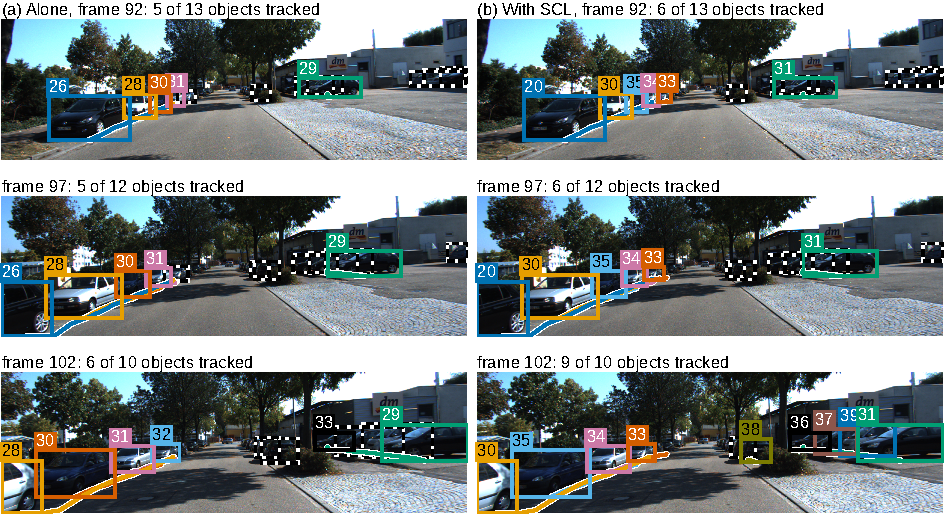
\includegraphics[width=0.98\textwidth]{figures/scl_kitti_example.pdf}
\caption{Tracking on KITTI sequence 0001 \cite{geiger2012kitti} with OC-SORT and YOLOv8n, at frames 92, 97, and 102 (rows): (a) the tracker alone, (b) with SCL. Each output track keeps one ID and one colour over the frames; the line of the same colour is its path over the previous 20 frames (bottom centre of its box). Dashed boxes: labelled objects that no track covers. IDs are numbered separately in each run. The sequence has the median HOTA gain of the 21 sequences, and frame 102 is its first frame with the largest gain in tracked objects.}
\label{fig:res-scl-example}
\end{figure}

\subsection{Evaluation under Shifted Detector Scores}\label{sec:res-shift}
Table~\ref{tab:res-scl-shift} shows the trackers under the four score transforms. Halving the scores reduced ByteTrack (official setting) and OC-SORT to 0 HOTA; with the layer they reached 66.17 and 66.72. Cubing reduced them to 60.92 and 58.34, and the layer restored them to 65.81 and 66.60; BoostTrack rose from 61.33 to 64.84. With $T=2$, the layer raised ByteTrack and OC-SORT by 1.11 and 1.24 points. The library setting of ByteTrack, whose low thresholds already accept the changed scores, stayed within 0.14 points. Over the 14 conditions, the layer raised HOTA significantly in 7 and lowered it significantly in none.

\begin{table}[tbp]
\centering
\caption{Baseline comparison under shifted detector scores on MOT17 val-half. The detector scores are transformed before the tracker, whose published thresholds stay fixed; $T$ is a logit temperature, $\sigma(z/T)$. Host: the tracker alone, without SCL. $\Delta$: with SCL minus host, with 95\% paired-bootstrap interval (10,000 resamples, seed 42); bold intervals exclude zero. Emission floor 0.01 (BoostTrack 0.1).}
\label{tab:res-scl-shift}
\begin{tabular}{lrrl}
\toprule
 & \multicolumn{3}{c}{HOTA (\%)}\\
Transform & Host & + SCL & $\Delta$ [95\% CI]\\
\midrule
\multicolumn{4}{l}{\textit{ByteTrack, official setting} \cite{zhang2022bytetrack}}\\
\quad $s^3$ & 60.92 & 65.81 & \textbf{$+4.89$ [$+2.60$, $+13.69$]}\\
\quad $0.5\,s$ & 0.00 & 66.17 & \textbf{$+66.17$ [$+49.32$, $+75.40$]}\\
\quad $T=2$ & 65.84 & 66.95 & \textbf{$+1.11$ [$+0.35$, $+3.87$]}\\
\quad $T=0.5$ & 67.30 & 67.29 & $-0.009$ [$-0.051$, $+0.005$]\\
\multicolumn{4}{l}{\textit{ByteTrack, library setting} \cite{zhang2022bytetrack}}\\
\quad $s^3$ & 66.31 & 66.31 & $-0.006$ [$-0.384$, $+0.383$]\\
\quad $0.5\,s$ & 66.61 & 66.48 & $-0.14$ [$-0.66$, $+0.14$]\\
\quad $T=2$ & 63.97 & 63.97 & 0 (identical)\\
\quad $T=0.5$ & 66.53 & 66.52 & $-0.006$ [$-0.029$, $+0.001$]\\
\multicolumn{4}{l}{\textit{OC-SORT} \cite{cao2023ocsort}}\\
\quad $s^3$ & 58.34 & 66.60 & \textbf{$+8.26$ [$+5.86$, $+16.81$]}\\
\quad $0.5\,s$ & 0.00 & 66.72 & \textbf{$+66.72$ [$+50.32$, $+75.56$]}\\
\quad $T=2$ & 65.99 & 67.22 & \textbf{$+1.24$ [$+0.52$, $+3.42$]}\\
\quad $T=0.5$ & 66.61 & 67.06 & $+0.45$ [$-0.01$, $+0.97$]\\
\multicolumn{4}{l}{\textit{BoostTrack, online} \cite{stanojevic2024boosttrack}}\\
\quad $s^3$ & 61.33 & 64.84 & \textbf{$+3.51$ [$+0.85$, $+13.28$]}\\
\quad $T=2$ & 67.59 & 67.59 & 0 (identical)\\
\bottomrule
\end{tabular}
\end{table}

\subsection{Frozen Evaluation on External Trackers}\label{sec:res-scl-external}
Table~\ref{tab:res-scl-external} gives the two predeclared external systems. PD-SORT \cite{wang2025pdsort} was reproduced exactly. With SCL, its HOTA rose by 0.61 points ([$+0.27$, $+1.65$]), its MOTA by 1.13 ([$+0.27$, $+3.03$]), and its IDF1 by 0.82 ([$+0.43$, $+1.94$]), with higher HOTA on 7 of 7 sequences; like OC-SORT, it is a single-stage tracker, but it was not seen during design. Hybrid-SORT \cite{yang2024hybridsort}, a two-stage tracker, gave identical output, as predicted before the run.

\begin{table}[tbp]
\centering
\caption{Baseline comparison on the predeclared external systems (MOT17 val-half, authors' released detections), each evaluated once with the frozen SCL. Paper: number reported by the authors (for PD-SORT, their released output). Host: the tracker alone, without SCL (our run of the published tracker). Reproduction class against the authors' number (EXACT: $|\Delta\mathrm{HOTA}|\le0.2$; CLOSE: $\le1.0$ with a documented, untuned cause). $\Delta$: host with SCL minus host, with 95\% paired-bootstrap interval; bold intervals exclude zero. IDS: identity switches, a count (lower is better); --: not reported.}
\label{tab:res-scl-external}
\begin{tabular}{lrrl}
\toprule
Metric & Paper & Host & $\Delta$ [95\% CI]\\
\midrule
\multicolumn{4}{l}{\textit{PD-SORT} \cite{wang2025pdsort}\textit{, EXACT}}\\
\quad HOTA & 68.01 & 68.01 & \textbf{$+0.61$ [$+0.27$, $+1.65$]}\\
\quad MOTA & 75.19 & 75.19 & \textbf{$+1.13$ [$+0.27$, $+3.03$]}\\
\quad IDF1 & 81.03 & 81.03 & \textbf{$+0.82$ [$+0.43$, $+1.94$]}\\
\quad IDS & -- & 129 & $+2$ [$-9$, $+13$]\\
\multicolumn{4}{l}{\textit{Hybrid-SORT} \cite{yang2024hybridsort}\textit{, CLOSE}}\\
\quad HOTA & 67.1 & 66.70 & 0 (identical)\\
\quad MOTA & 75.8 & 75.52 & 0 (identical)\\
\quad IDF1 & 78.0 & 77.56 & 0 (identical)\\
\quad IDS & -- & 259 & 0 (identical)\\
\bottomrule
\end{tabular}
\end{table}

\subsection{Frozen UAVDT Transfer}\label{sec:res-scl-uavdt}
On the held-out UAVDT test split (Table~\ref{tab:res-scl-uavdt}), SCL raised the HOTA of the YOLOv8n stream by 1.77 points ([$+0.70$, $+2.94$]) and its IDF1 by 3.97 points, and cut identity switches by 45\%. With RT-DETR-L, whose host produced many false positives (MOTA 3.29), SCL raised MOTA by 24.70 points ([$+10.06$, $+51.08$]) and IDF1 by 5.74 points, and cut false positives by 58\% and identity switches by 56\%. No HOTA decrease was detected with either detector.

\begin{table}[tbp]
\centering
\caption{Baseline comparison on the held-out UAVDT test split (20 aerial sequences, not used during design), evaluated once with the frozen SCL. Host: ByteTrack alone, without SCL, with its published setting. $\Delta$: host with SCL minus host, with 95\% paired-bootstrap interval; bold intervals exclude zero. IDS: identity switches, a count (lower is better).}
\label{tab:res-scl-uavdt}
\begin{tabular}{lrl}
\toprule
Metric & Host & $\Delta$ [95\% CI]\\
\midrule
\multicolumn{3}{l}{\textit{ByteTrack, RT-DETR-L} \cite{zhang2022bytetrack,zhao2024rtdetr}}\\
\quad HOTA & 40.07 & $+2.30$ [$-1.05$, $+6.55$]\\
\quad MOTA & 3.29 & \textbf{$+24.70$ [$+10.06$, $+51.08$]}\\
\quad IDF1 & 48.59 & \textbf{$+5.74$ [$+0.13$, $+13.11$]}\\
\quad IDS & 1041 & \textbf{$-586$ [$-951$, $-248$]}\\
\multicolumn{3}{l}{\textit{ByteTrack, YOLOv8n} \cite{zhang2022bytetrack,jocher2023yolov8}}\\
\quad HOTA & 29.05 & \textbf{$+1.77$ [$+0.70$, $+2.94$]}\\
\quad MOTA & 16.27 & $+1.02$ [$-1.06$, $+2.86$]\\
\quad IDF1 & 34.52 & \textbf{$+3.97$ [$+1.88$, $+6.17$]}\\
\quad IDS & 719 & \textbf{$-326$ [$-691$, $-73$]}\\
\bottomrule
\end{tabular}
\end{table}

\subsection{Runtime of SCL}\label{sec:res-scl-runtime}
SCL needs no training, no GPU, and no access to the inside of the detector or the tracker. On the CPU of Table~\ref{tab:res-env} it takes 2.95 ms per frame, small next to the 42 ms of the detector, and the tracker itself ran faster with it (1.43 against 2.04 ms per frame); the end-to-end time rose by only 4.5\%. A new tracker is added through its four published contract values and an adapter, without changes to the rules.

\section{Comparison with Existing Approaches}\label{sec:res-compare}

\subsection{Comparison with Adaptive-Threshold Baselines}\label{sec:res-baselines}
Two simple baselines set the tracker's matching and birth thresholds in every frame to the first or second Otsu split of the logits of the last 10 frames, $t_1$ or $t_2$, and pass the scores unchanged. On KITTI (Table~\ref{tab:res-baselines}), SCL reached the highest HOTA in all three cells, 2.2 to 8.6 points above the baselines, with intervals against the $t_2$ baseline above zero in every cell, so adaptive thresholds alone do not explain the gains. With OC-SORT, SCL also had fewer identity switches than both baselines (170 against 1,545 and 250 with YOLOv8n; 308 against 1,975 and 492 under halved scores).

\begin{table}[tbp]
\centering
\caption{HOTA (\%) of SCL and of two simple adaptive-threshold baselines on KITTI tracking training (official HOTA, car and pedestrian averaged). Host: the tracker alone, without any layer. $t_1$, $t_2$: the adaptive baselines, in which the tracker's matching and birth thresholds are set in every frame to the first or second Otsu split of the logits of the last 10 frames, and the scores are passed unchanged. Halved: halved detector scores. $\Delta$: SCL minus the $t_2$ baseline, with 95\% paired-bootstrap interval; bold intervals exclude zero.}
\label{tab:res-baselines}
\begin{tabular}{lrrrrl}
\toprule
Cell & Host & $t_1$ & $t_2$ & SCL & $\Delta$ [95\% CI]\\
\midrule
OC-SORT, YOLOv8n & 36.27 & 39.97 & 41.09 & 44.17 & \textbf{$+3.09$ [$+2.00$, $+4.03$]}\\
ByteTrack, RT-DETR-L, halved & 49.50 & 49.58 & 49.50 & 51.78 & \textbf{$+2.29$ [$+0.28$, $+4.96$]}\\
OC-SORT, YOLOv8n, halved & 0.00 & 37.68 & 43.56 & 46.30 & \textbf{$+2.74$ [$+1.32$, $+3.34$]}\\
\bottomrule
\end{tabular}
\end{table}

\subsection{Comparison with ACT}\label{sec:res-act}
ACT \cite{act2026adaptive} was run with its published parameters, without retuning, on the same detections (Table~\ref{tab:res-act}). SCL reached higher HOTA than ACT in every row, significantly under halved scores ($+2.01$ and $+10.06$ points) and with YOLOv8n on UAVDT ($+1.82$), and also in the MOT17 setting for which ACT was designed. With RT-DETR-L on UAVDT, SCL reached a MOTA of 27.99 against 5.34 ($+22.65$, [$+9.03$, $+47.21$]), because the fixed score levels of ACT removed few of the host's false positives (178,219 against 78,975). SCL also had fewer identity switches than ACT on MOT17 and UAVDT (up to 418 fewer).

\begin{table}[tbp]
\centering
\caption{HOTA of ACT and of SCL on the same detections, and the differences SCL minus ACT in HOTA and IDF1, with 95\% paired-bootstrap interval; bold intervals exclude zero. ACT: published parameters, no tuning. KITTI: official HOTA, car and pedestrian averaged; MOT17: val-half, ACT's own setting; UAVDT: test split, one vehicle class, ignored regions removed.}
\label{tab:res-act}
\begin{tabular}{>{\raggedright\arraybackslash}p{2.3cm}>{\raggedright\arraybackslash}p{1.8cm}>{\raggedright\arraybackslash}p{2.1cm}rr>{\raggedright\arraybackslash}p{2.6cm}>{\raggedright\arraybackslash}p{2.6cm}}
\toprule
Data & Detector & Tracker & ACT & SCL & $\Delta$HOTA & $\Delta$IDF1\\
\midrule
KITTI, halved scores & RT-DETR-L & ByteTrack & 49.77 & 51.78 & \textbf{$+2.01$ [$+0.01$, $+4.76$]} & $+1.70$ [$-1.13$, $+6.80$]\\
KITTI, halved scores & YOLOv8n & OC-SORT & 36.24 & 46.30 & \textbf{$+10.06$ [$+6.88$, $+12.01$]} & \textbf{$+12.03$ [$+6.85$, $+14.69$]}\\
MOT17, floor 0.01 & YOLOX-X & ByteTrack (official) & 67.46 & 67.68 & $+0.22$ [$-0.43$, $+0.88$] & $+0.57$ [$-0.68$, $+2.12$]\\
MOT17, floor 0.1 & YOLOX-X & ByteTrack (official) & 67.46 & 67.70 & $+0.23$ [$-0.40$, $+0.90$] & $+0.60$ [$-0.55$, $+2.10$]\\
UAVDT test & YOLOv8n & ByteTrack & 29.01 & 30.83 & \textbf{$+1.82$ [$+0.65$, $+3.00$]} & \textbf{$+4.00$ [$+1.85$, $+6.22$]}\\
UAVDT test & RT-DETR-L & ByteTrack & 40.14 & 42.37 & $+2.23$ [$-0.97$, $+6.32$] & $+5.35$ [$-0.03$, $+12.47$]\\
\bottomrule
\end{tabular}
\end{table}

\subsection{Contribution of Each Part of SCL}\label{sec:res-parts}
Removing one part at a time on KITTI shows where the gains come from: without the rescue, HOTA fell by up to 3.35 points; without the mode decision, by up to 2.44; and without the new scores of the noisy mode, by up to 1.67. Each part therefore contributes to the result, and the rescue contributes most.

\subsection{Comparison of Properties}\label{sec:res-properties}
Table~\ref{tab:res-properties} compares the proposed controllers with the closest adaptive methods by what they adapt, where they act, and for which task they are designed. AC-MOT is the only method in the table that adapts the confidence threshold, the NMS threshold, and the input resolution of the detector together for tracking, with the tracker unchanged. SCL is the only one that serves several unchanged trackers through their published thresholds and decides from the score distribution of past frames whether to act at all.

\begin{table}[tbp]
\centering
\caption{Adaptive methods closest to the proposed controllers.}
\label{tab:res-properties}
\begin{tabular}{>{\raggedright\arraybackslash}p{3.4cm}>{\raggedright\arraybackslash}p{4.2cm}>{\raggedright\arraybackslash}p{3.9cm}>{\raggedright\arraybackslash}p{2.9cm}}
\toprule
Method & Adapted & Where & Task\\
\midrule
AdaScale \cite{chin2019adascale} & input scale & detector & video detection\\
ApproxDet \cite{xu2020approxdet} & detection configuration & detector & video detection\\
Chameleon \cite{jiang2018chameleon} & pipeline configuration & analytics pipeline & video analytics\\
Adaptive ByteTrack \cite{ma2023adaptivebytetrack} & confidence threshold & inside ByteTrack & MOT\\
AdapTrack \cite{shim2024adaptrack} & matching thresholds & inside the tracker & MOT\\
ACT \cite{act2026adaptive} & high and low thresholds from the current scores & tracker thresholds & MOT\\
AC-MOT (this thesis) & confidence, NMS, resolution & detector; tracker unchanged & aerial MOT\\
SCL (this thesis) & candidates, scores, thresholds, matching tolerance & between detector and tracker; both unchanged & MOT, several trackers\\
\bottomrule
\end{tabular}
\end{table}

\section{Discussion}\label{sec:res-discussion}

\emph{The operating point is part of the MOT system.} The same frozen detector and trackers give very different MOT results at different operating points: moving away from the fixed 1536/0.70 point raises MOTA by 17.995 points with ByteTrack and by 6.318 points with OATrack on VisDrone. On both aerial datasets FP and IDS drop sharply and precision rises, while FN rise a little, so MOTA, which counts every FP, reacts most strongly. The detector operating point is therefore a first-order variable of aerial MOT and deserves the same attention as the association method.

\emph{The score scale is part of the MOT system.} Halving the scores reduced ByteTrack and OC-SORT from 67.70 and 66.43 HOTA to 0, and with RT-DETR-L on UAVDT ByteTrack reached a MOTA of only 3.29. The fixed thresholds of a tracker hold only for the detector they were tuned for, so the score scale deserves the same attention as the association method.

\emph{Tracker dependence.} With AC-MOT, ByteTrack, which starts from a weaker baseline and uses low-score boxes in its second association step, gains more than OATrack, which already weights detections by quality and gains mainly in MOTA, IDF1, IDS, and FP. With SCL, single-stage trackers gain through the rescue, and two-stage trackers gain when the detector is noisy. The best adaptation therefore depends on the tracker host, and both controllers serve the host without changing it.

\emph{Self-limiting by design.} In the clean mode SCL keeps the tracker's thresholds and scores, so a well-matched tracker receives its normal input; AOB, which always intervened, lowered the same trackers by 4.15 to 5.89 HOTA points. AC-MOT keeps its state changes rare through its window, holds, and dwell rule, so the detector input stays stable over long stretches of video.

\emph{Deployment.} Neither controller needs training, labels, or access to the inside of the detector or the tracker. AC-MOT changes three arguments of the detector call and takes about 4.2 ms per frame on a Tesla T4; SCL runs on a CPU in 2.95 ms per frame. Table~\ref{tab:res-summary} summarizes the two controllers.

\begin{table}[tbp]
\centering
\caption{Summary of the two proposed controllers.}
\label{tab:res-summary}
\begin{tabular}{>{\raggedright\arraybackslash}p{2.8cm}>{\raggedright\arraybackslash}p{5.8cm}>{\raggedright\arraybackslash}p{5.8cm}}
\toprule
Aspect & AC-MOT & SCL\\
\midrule
Acts on & detector operating point: confidence threshold, NMS threshold, input resolution & tracker input: candidates, scores, thresholds, matching tolerance\\
Reads & image cues of the current frame and tracked boxes of the previous frame & score logits of the last 10 frames, tracks of the previous frame, camera motion\\
Update & every 10 frames & every frame\\
Decision & three states from the scene complexity index, with recovery, hysteresis, and dwell & clean or noisy mode from nested Otsu splits and a whole-stream median\\
Values chosen by & cross-validation on calibration sequences & standard values and design choices, no search\\
Evaluated on & VisDrone2019-MOT and UAVDT with ByteTrack and OATrack & MOT17, KITTI, and UAVDT with seven published trackers\\
Main results & VisDrone: HOTA $+2.937$ and $+1.325$, MOTA $+17.995$ and $+6.318$; UAVDT: MOTA $+17.601$ and $+3.267$ & halved scores: 0 to 66.17 and 66.72 HOTA; KITTI: MOTA $+5.98$ and $+7.86$; UAVDT: MOTA $+24.70$\\
Cost & 4.26 and 4.20 ms per frame (Tesla T4) & 2.95 ms per frame (CPU)\\
\bottomrule
\end{tabular}
\end{table}
